%%%%%%%%%%%%%%%%%%%%%%%%%%%%%%%%%%%%%%%%%%%%%%%%%%%%%%%%%%%%%%%%%%%%%%%%%%%%%%%%
%2345678901234567890123456789012345678901234567890123456789012345678901234567890
%        1         2         3         4         5         6         7         8

\documentclass[letterpaper, 12 pt, conference]{ieeeconf}  % Comment this line out
                                                          % if you need a4paper
%\documentclass[a4paper, 10pt, conference]{ieeeconf}      % Use this line for a4
                                                          % paper

\IEEEoverridecommandlockouts                              % This command is only
                                                          % needed if you want to
                                                          % use the \thanks command
\overrideIEEEmargins
% See the \addtolength command later in the file to balance the column lengths
% on the last page of the document


\usepackage{fullpage}
\usepackage{graphicx}
\usepackage[colorinlistoftodos]{todonotes}
\usepackage{hyperref}

% The following packages can be found on http:\\www.ctan.org
\usepackage{graphicx} % for pdf, bitmapped graphics files
\usepackage{bm}
\newcommand{\uvec}[1]{\boldsymbol{\hat{\textbf{#1}}}}
%\usepackage{epsfig} % for postscript graphics files
%\usepackage{mathptmx} % assumes new font selection scheme installed
%\usepackage{times} % assumes new font selection scheme installed
%\usepackage{amsmath} % assumes amsmath package installed
%\usepackage{amssymb}  % assumes amsmath package installed

\title{\LARGE \bf
Using Artificial Neural Networks for Instrument Classification of Audio Signals
}


\author{Saksham Goel% <-this % stops a space
%\thanks{}% <-this % stops a space
%\thanks{$^{1}$Saksham Goel, Student - Department of Computer Science, University of Minnesota - Twin Cities}%
}


\begin{document}

\maketitle
\thispagestyle{empty}
\pagestyle{empty}

%%%%%%%%%%%%%%%%%%%%%%%%%%%%%%%%%%%%%%%%%%%%%%%%%%%%%%%%%%%%%%%%%%%%%%%%%%%%%%%%
% ABSTRACT
%%%%%%%%%%%%%%%%%%%%%%%%%%%%%%%%%%%%%%%%%%%%%%%%%%%%%%%%%%%%%%%%%%%%%%%%%%%%%%%%
\begin{abstract}
This project examines the applications of using different types of Deep Learning Architectures like Recurrent Neural Networks (RNN) and Convolutional Neural Networks (CNN) for instrument recognition from an audio sample. The project is divided into two section. First section of the project explores the time dependency of the audio signals hence uses architectures like Simple Vanilla RNN, Gated Recurrent Unit (GRU) \cite{gru_translation}, Long Short Term Memory (LSTM) \cite{lstm_sequence_modelling} \cite{lstm_music_genre} and Bidirectional Long Short Term Memory (BLSTM) \cite{bidirectional_lstm_speech}. All these architectures try to learn feature representation from the given input audio file dependent on the values before (in case of BLSTM also after) the current timestep. Because audio data is just like time series data, these techinques are being used and will be compared to see which architecture performs the best in the field of instrument recognition. Second section on the contrary explores the local dependency of the audio signals, attempting to recognize overtones, and hence applies CNN architecture on various two dimensional representation of the given audio data. For the purpose of this project we are considering two types 2-Dimensional representations of the Audio Data: Stacking and Multiresolution Recurrence Plots (MRP) \cite{cnn_music_mrp}. Other than this, we will also be trying to apply a technique of exploiting local and time dependent features by using architectures that combine the characterstics of RNN's and CNN's \cite{cnn_rnn_sleep_staging} \cite{crnn} and compare their results.
\end{abstract}
%%%%%%%%%%%%%%%%%%%%%%%%%%%%%%%%%%%%%%%%%%%%%%%%%%%%%%%%%%%%%%%%%%%%%%%%%%%%%%%% 
%%%%%%%%%%%%%%%%%%%%%%%%%%%%%%%%%%%%%%%%%%%%%%%%%%%%%%%%%%%%%%%%%%%%%%%%%%%%%%%%




%%%%%%%%%%%%%%%%%%%%%%%%%%%%%%%%%%%%%%%%%%%%%%%%%%%%%%%%%%%%%%%%%%%%%%%%%%%%%%%%
% INTRODUCTION
%%%%%%%%%%%%%%%%%%%%%%%%%%%%%%%%%%%%%%%%%%%%%%%%%%%%%%%%%%%%%%%%%%%%%%%%%%%%%%%%
\section{\textbf{Introduction}}

%Our problem is the classification/identification of an instrument based on a sound snippet in the form of a stereo sound. For solving this problem we will be using the Instrument Recognition in Music Audio Signals (IRMAS) Dataset \cite{bosch2012comparison}. The problem statement in a more formal sense is as follows: Given an audio excerpt which contains some musical audio with a predoiminated sound of a given instrument, need to classify 3 second windows of that given audio excerpt into one category from any of the following category: "Cello", "Clarinet", "Flute", "Acoustic Guitar", "Electric Guitar", "Organ", "Piano", "Saxophone", "Trumpet", "Violin", and "Human Singing Voice". For this problem, we hope to solve the problem using different machine learning algorithms. The focus for this project would be to use different Deep Learning Architectures used in Image Classification, Sequence Modelling and Speech Recognition to classify the audio files. The primary architectures that are being considered include Convolutional Neural Networks (CNN), Recurrent Neural Networks (RNN).



Music is one of the most popular source of entertainment for us humans and boasts one of the biggest entertainment industries. A lot of research is being done currently for novel ways of queriying music and sound signals. These ways focus on being able to query audio signals based on various parameters like: similarity to other music, recommendation based on user activity, instrument, music genre, music pace etc. These novel ways help improve the user experience drastically and also help in efficient retrieval of the required audio samples. However annotating all the audio sample via human labor is very expensive and time consuming. This project aims to set up a proof of concept for using different deep learning architectures for the task of instrument classification of audio signals so that it can be used to automatically label sound recordings. This project focuses on training different deep learning architectures as mentioned in the abstract and performing a comparison of the accuracies. The problem statement is: \textit{Given an audio signal with a dominated sound of a given instrument, the model will classify some $t$ second sliding windows of that given audio excerpt into one category from any of the following categories mentioned in Table \ref{tab:pd}.}

\begin{table}[!h]
\centering
\caption{Number of Training Samples by Instrument Class}
\begin{tabular}{| c || c |} %sets the format of the table
\hline %horizontal line
 Instrument Category &  Number of Audio Files \\
   \hline \hline
\hline
Electric Guitar &  760 \\
\hline
Piano  &   721 \\
\hline
Saxophone  &   626 \\
\hline
Violin &   580 \\
\hline
Human Singing Voice  &   778 \\
\hline
   \end{tabular}
\label{tab:pd} 
\end{table}

With novel approaches that can automatically start extracting information from audio datasets, we can not only query audio data efficiently and effectively, but also develop several models that can help develop different types of music which are more personally centered based on a users activity etc. Also once these kinds of models have been developed, they can be used to automatically generate user profiles from their music history which can be used to provide better recommendations, understand user's current mood, profile user's activity and much more. Also, companies like YouTube, Spotify can use these kind of technoligies to create a vast database for their sound and video database to add more features without spending money on any kind of human labor. Also, considering how digital assitants like Google Home, Apple Siri, Amazon Alexa. are becoming more prevelant in households today, these types of techonlogies can also help them differentiate between music and human audio and thus help them be better listener when there is music playing in the background.
%%%%%%%%%%%%%%%%%%%%%%%%%%%%%%%%%%%%%%%%%%%%%%%%%%%%%%%%%%%%%%%%%%%%%%%%%%%%%%%%
%%%%%%%%%%%%%%%%%%%%%%%%%%%%%%%%%%%%%%%%%%%%%%%%%%%%%%%%%%%%%%%%%%%%%%%%%%%%%%%%




%%%%%%%%%%%%%%%%%%%%%%%%%%%%%%%%%%%%%%%%%%%%%%%%%%%%%%%%%%%%%%%%%%%%%%%%%%%%%%%%
% RELATED WORK
%%%%%%%%%%%%%%%%%%%%%%%%%%%%%%%%%%%%%%%%%%%%%%%%%%%%%%%%%%%%%%%%%%%%%%%%%%%%%%%%
\section{\textbf{Related Work}}
Audio recognition is very widely researched filed in todays time. A lot of research is being conducted in the field of speech recognition to make the existing digital assitants like Siri, Google Home better and much more accurate. Most of the research currently focuses on applying different types of traidtional machine learning and deep learning algorithms to process the audio data and get the desired output. However unlike other forms of data, audio data is unstructured data. Also, audio data is very special because of its inherent structure which dictates dependency between sound signals at two different signals. Audio signals are temporal data much like time series data such that they have long range dependency between signals at two different timesteps. Because of this property it is very hard to achieve great performance through traditional machine learning algorithms on raw audio data. Traidtional machine learning algorithms assume that the features of the data are independent and identically distributed, which is not true when dealing with raw audio data	. Even the traditional artificial neural networks are not designed to use previous information to influence their decision for the current input. They assume the given input features are independent of one other. This assumption is not valid in scenarios handling raw audio data. This is why this project focuses on working with different deep learning architectures like Recurrent Neural Networks (RNN) and Convolutional Neural Networks (CNN) because of their promising results in the fields of audio and image processing.

RNNs are a special type of artifical neural network designed specifically for handling time series data or data where the inputs are dependent on each other. RNNs are one of the most popular deep learning architecture used in the field of dependent values and modeling time series like data is RNN. They address the issue of dependence among feature values, by inserting loops in them as can be seen in Figure: \ref{fig:RNN_Loop}, which allows information to persist. 

\begin{figure}[!h]
\centering
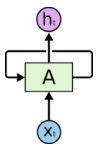
\includegraphics[scale=0.7]{../figs/rnn/loop.png}	
\caption{Input Output loop in RNN}
\label{fig:RNN_Loop} 
\end{figure}

Chung et al \cite{gru_evaluation} mentions that because of this property, RNNs have been widely used in the fields of sequence modelling and have proven successful. Also as mentioned in Sak	et al \cite{google_accoustics} \cite{google_speech}, RNN's have proven successful in modelling natural language and speech processing. RNNs are also very powerful than some of its other counterparts like ANNs and CNNs because unlike them, the dimensions of the input and output vectors for RNNs can be of arbitrary dimension	 \cite{gru_evaluation}, depending on the length of the sequence itself.

\begin{figure}[!h]
\centering
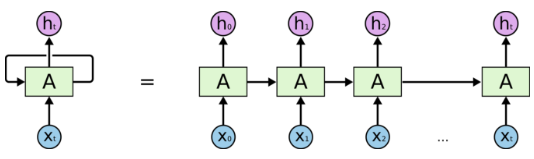
\includegraphics[scale=0.5]{../figs/rnn/unrolled.png}	
\caption{Unrolled Recurrent Neural Network}
\label{fig:RNN_Unrolled} 
\end{figure}

The motivating idea behind RNN is to process a set of input value and store some information derived from it in its own memory called the internal or hidden state. The internal state is updated at every time step using different weight matrices and activation functions depending on the type of architecture used. Cho et al \cite{gru_translation}, specifies that the internal state of the cell is dependent on the current timestep input and internal state from the previous timestep, however the output value of the current timestep is calculated using the current internal state. This kind of relationship can be formulated mathematically as follows:
\begin{equation}
h_t = f(x_t, h_{t-1})
\end{equation}

Here $h_t$ represents the internal state of the current cell or $t^{th}$ cell, $x_t$ represents the $t^{th}$ input and $h_{t-1}$ represents the ${t-1}^{th}$ cell's internal state. This kind of relationship among the input, internal and output values in a RNN cell is what makes them very apt for modeling the intricate dependencies in a time series.

Apart from traditional Vanilla RNNs, there are two other types of RNNs that have been studied at extent. One of them is called Long Short-Term Memory Recurrent Neural Network which features a block named LSTM unit which was introduced by Hochreiter et al \cite{lstm_intro}. LSTM was developed to overcome the problem of Vanishing Gradients in Vanilla RNN which was discovered by Pascanu et al\cite{vanishing_gradient} and Hochreiter et al \cite{lstm_intro}. Because of this property LSTM has been very successful in modelling long term dependencies and proved very effective in generating sequence as mentioned in Graves et al \cite{lstm_sequence_modelling}. Also, according to the experiments conducted by Tang et al \cite{lstm_music_genre} and Herrera-Boyer et al \cite{audio_classification} LSTM has been successful in modelling audio data for achieving classification tasks on instruments and music genre. The other architecture is called Gated Recursive Neural Network which features a block named Gated Recurrent Unit (GRU) which is extensivley used in fields of machine translation \cite{gru_translation}. While LSTM was developed based off Vanilla RNN model to overcome the problem of vanishing gradients, GRU was developed by Cho et al \cite{gru_translation} and was based on the LSTM model. It was developed to overcome the problems of slower convergence and drastically high number of parameters in the LSTM model. In terms of performance LSTM has higher accuraccy because of large number of parameters, however it is easier to train GRU networks without much loss in accuraccy. 

LSTM is also very popular in modelling accoustic data as used by Google \cite{google_accoustics}. The architectures used by Google for accoustic modelling \cite{google_accoustics} are LSTM RNN, Deep Long Short-Term Memory (DLSTM) RNN, Long Short-Term Memory Projected (LSTMP) RNN and Deep Long Short-Term Memory Projected (DLSTMP) RNN to combat various problems like Vanishing Gradients, Long Range Dependency between temporal sequences and also to combat the huge number of learnable parameters. The DLSTM essentially repeats the number of LSTM units so that there can different learnable parameter matrices. This helps to learn different reoresentations from the same audio data and hence could be useful and worth a try. The latter two types of RNN mentioned are specifically designed to preserve as much information while essentially decreasing the number of parameters by adding a linear projection layer \cite{google_accoustics} after each LSTM unit. Because of this reduction in number of parameters, it promises less computation and faster convergence while having similar performance.

Another type of RNN architecture is a Bidirectional LSTM. It is different from the previous architectures because they all extract information from the previous context or from past. However sometimes it is better to use the information from past and future context at once. Yu et al \cite{blstm_intro} mentions that when modelling english language, sometimes it is helpful to extract information from past and the future context to remove ambiguity. BLSTM implement this kind of behavior by connecting two hidden layers of opposite directions to the same output \cite{blstm_intro}. BLSTM have been proven useful when the context of the input is crucial for the performance, for example, in handwriting recognition, speech recognition \cite{bidirectional_lstm_speech}, speech synthesis, phenome classification and protein synthesis \cite{blstm_protein}.


%Other than that the architecture some researchers used for speech recognition \cite{graves2014towards} is a Bidirectional Long Short-Term Memory (BLSTM) RNN. A BLSTM, differs from the previous known architectures in the form that it uses both the previous time stamps hidden state and the future timestamps hidden state along with the input value to calculate the current hidden state. In essence as compared to earlier models which only depend on the previous timestamps (just information from past) while BLSTM takes into account the information from both the past and future values. In this manner BLSTM are able to better understand the context and eliminate ambiguity. We are trying to train a BLSTM just to check whether it performs better then other models, and if it does then why might it be doing that, so that we can better understand the music audio data in light of classification of instruments.

%The advantage of using LSTM architecture is that LSTM is very good at solving the problem of vanishing gradients when the data has very long temporal dependencies. With the inclusion of different gates (inherent computations to calculate the hidden state) like memory and forget gates which affect the computation of the hidden state, LSTM essentially can use the values to include the memory from previous timesteps and influence the output accordingly, hence effectively capturing long distance temporal dependencies. On the other hand GRU is very much similar to LSTM using different gates, but has a different architecture for the GRU unit. GRU combines some of the gates in LSTM cell (like forget and input gate) to essentially reduce the number of learnable parameters. Due to this, both of them differ in the way they let the output affect the memory inclusion, and also how the output value is calculated \cite{chung2014empirical}, while trying to solve the same problem of long term temporal dependencies. The advantage of GRU over LSTM is that it used smaller set of learnable parameters and hence is easier to train and expected to reach a state of convergence much faster. On the other hand advantages of LSTM is that they can learn more abstract long term dependencies because of their intricate structure. Considering that the audio data has a high number of features (a lot of sound signals in the 3 second window \textbackslash 1.2 Million sound signals per 3 second window) it will be good to use GRU so that we can essentially train the model easily and reach convegence early, however LSTM may proove to be more accurate.


Other than RNN for this project we will also be trying to apply Convolutional Neural Networks (CNN) on our problem. CNNs were designed specifically for the purpose of processing visual data like images. In today's time, CNN based architectures have been widely used in fields like Image Classification \cite{ilsvrc} and Object Detection. As Krizhevsky et al \cite{imagenet_original} demonstrates, the motivating idea behind CNNs is that visual data has an inherent local structure such that values which are closer to each other tend to influence each other. To understand this, we can take the example of an image of a scenery. We know pixels representing the grass in the image tend to be similar to each other (mostly green). 


CNNs are very powerful tool because they automatically learn different latent visual features also termed as \textit{"feature maps"} from the input image. This property makes CNN's very different from other traditional Machine Learning Algorithms, where the features have to be already specified. Considering the CNN's learn these high dimensional feature maps from the given input we aim to use CNNs to extract these features and then build a neural network model on top of these features to classify the audio dataset. According to experiments performed by Park et al \cite{cnn_music_mrp} CNNs performed very well on Multiresolution Recurrence Plot images of audio data. CNNs have also been used along with RNNs in an effort to extract the features from images and then extract information from the time series component. This kind of idea was used in Agarwal et al \cite{cnn_rnn_sleep_staging} for modelling sleep stages and by Choi et al \cite{crnn} for instrument and music genre classification.

%CNN's have been used extensively in the field of Computer Vision for tasks like Image Classification \cite{krizhevsky2012imagenet} and Object Detection. Their popularity in the field of computer vision arises from the fact that they are very good at extracting/learning different high dimensional features from the input images. Convolutional Neural Networks use as the name suggests, a method called Convolution. Convolution refers to using feature maps/filters that are convolved (slided) on top of the input feature matrices to result into output feature matrices. This kind of convolution property helps them learn various high dimensional features which is the strength of the CNN. This property makes CNN's very different from other traditional Machine Learning Algorithms, where the features have to be already specified. Considering the CNN's learn these high dimensional feature maps from the given input we aim to use CNNs to extract these features and then build a neural network model on top of these features to classify the audio dataset. Although primarily CNN's have not been used much in the field like speech recognition and sequence modelling, CNN's can still proove to be very powerful tools for feature extraction. We aim to use these extracted features from CNN from the given input image and try to either classify based on that. Also, another way is to use this extracted features as the initial hidden state for a Vanilla RNN model and try to use signal values from the audio with this hidden state initialization in the RNN model to further classify the given audio signal to an instrument class. The motivation for this method comes from \cite{aggarwalstructured}, where a RNN was used on top of the output of a CNN to model for both local and temporal dependcy of the input sleep staging data.

%To conclude, there has already been a lot of work using different Deep Learning Architectures in different problem domains, and thus we aim to try to apply these techniques and compare the result and try to gain a better understanding about which architecture seems to be the best fit and understand why that is the case.
%%%%%%%%%%%%%%%%%%%%%%%%%%%%%%%%%%%%%%%%%%%%%%%%%%%%%%%%%%%%%%%%%%%%%%%%%%%%%%%%
%%%%%%%%%%%%%%%%%%%%%%%%%%%%%%%%%%%%%%%%%%%%%%%%%%%%%%%%%%%%%%%%%%%%%%%%%%%%%%%%





%%%%%%%%%%%%%%%%%%%%%%%%%%%%%%%%%%%%%%%%%%%%%%%%%%%%%%%%%%%%%%%%%%%%%%%%%%%%%%%%
% APPROACH
%%%%%%%%%%%%%%%%%%%%%%%%%%%%%%%%%%%%%%%%%%%%%%%%%%%%%%%%%%%%%%%%%%%%%%%%%%%%%%%%
\section{\textbf{Approach}}

%For this project we are focusing on different types of deep learning architectures to do instrument classification. The architectures can be divided into two different major architecture types: RNN and CNN. We will be comparing 4 different types of RNN architectures as follows:

%\begin{description}
%	\item [$\bullet$ Simple Vanilla RNN (Figure: \ref{fig:Vanilla_RNN_Arch})]
%	\item [$\bullet$ Long Short Term Memory (Figure: \ref{fig:LSTM_Arch})]
%	\item [$\bullet$ Gated Recurrent Unit (Figure: \ref{fig:GRU_Arch})]
%	\item [$\bullet$ Bidirectional LSTM (Figure: \ref{fig:BLSTM_Arch})]
%\end{description}

For this project, we are considering several different types of architecture of RNNs for the problem and all of these architectures usally differ in the computations for the internal state and the output.

\subsection{Vanilla RNN}
Vanilla RNNs are the most basic form of RNNs. A Vanilla RNN cell as depicted in Figure \ref{fig:Vanilla_RNN_Arch}, only has one $\tanh$ layer to compute the internal state. This cell only comprises of two sets of computation, one for the internal state and one for the output. The feedforward equations for the Vanilla RNN cell are as follows:

\begin{equation}
h_{t} = \tanh(W_{hh}h_{t-1} + W_{xh}x_t)
\end{equation}
\begin{equation}
y_{t} = W_{hy}h_{t}
\end{equation}

Vanilla RNNs are easy to train because of less number of parameters overall and are easy to apply for problems like classification on top of a sequence of values. 

\begin{figure}[!h]
\centering
\includegraphics[scale=0.20]{../figs/vrnn/diagram.png}	
\caption{Vanilla RNN Cell Architecture}
\label{fig:Vanilla_RNN_Arch} 
\end{figure}

However, one of the biggest disadvantage of using Vanilla RNN is that they are not the best tools for modelling long sequences. Vanilla RNNs are prone to a phenomenen called Vanishing Gradients \cite{vanishing_gradient} \cite{lstm_intro}. Vanishing Gradients refer to the property when the gradient change for the weights in a neural networks are vanishingly small and start approaching the value $0$. Because of this problem the network effectively stops to train/learn. The problem of Vanishing Gradient stems from the fact that different activation functions like $\tanh$ have a gradient value in range: $(0, 1)$. When using the chain rule to calculate the gradient change in earlier layers, the continous multiplication of these small gradient values leads to an exponential decrease in gradient value leading to very small gradient updates.


\subsection{Long Short Term Memory (LSTM)}
Long Short Term Memory networks – usually just called “LSTMs” – are a special kind of RNN, capable of learning long-term dependencies. They were introduced by Hochreiter et al \cite{lstm_intro} to specifically model long term dependencies in a sequence and to combat the problem of vanishing and exploding gradients. Remembering information for long periods of time is practically their default behavior, unlike Vanilla RNN's which struggle to learn long term dependencies.

\begin{figure}[!h]
\centering
\includegraphics[scale=0.40]{../figs/lstm/diagram.png}	
\caption{LSTM Cell Architecture}
\label{fig:LSTM_Arch} 
\end{figure}

Unlike, Vanilla RNNs, LSTM cell \cite{lstm_intro} have four layers of networks interacting in a very special way as can be seen in Figure \ref{fig:LSTM_Arch}. This structure is what makes them combat the problem of vanishing gradient also makes them on the best choices for modelling accoustics \cite{google_accoustics} and for modelling speech \cite{google_speech}.

The key to LSTMs is the \textbf{cell state}, which is different from the hidden/internal state, the horizontal line running through the top of the diagram. This line ensures smooth back propogation of the gradient values by providing a bypass to the gradient values without becoming vanishingly small. Apart from the current cell state, LSTM also includes connections of its input through different gates called the forget, input and output gates. These gates determine what information is persisted, thrown away and added to the current cell state and the internal state. The interaction between the inputs and different gates can be mathematically written as follows:
\begin{equation}
f_{t} = \sigma(W_f\cdot[h_{t-1}, x_t] + b_f)
\end{equation}
\begin{equation}
i_{t} = \sigma(W_i\cdot[h_{t-1}, x_t] + b_i)
\end{equation}
\begin{equation}
\bar{C}_t = \tanh(W_C\cdot[h_{t-1}, x_t] + b_C)
\end{equation}
\begin{equation}
C_t = f_t \cdot C_{t-1} + i_t \cdot \bar{C}_t
\end{equation}
\begin{equation}
o_t = \sigma(W_o[h_{t-1}, x_t] + b_o)
\end{equation}
\begin{equation}
h_t = o_t \cdot \tanh(C_t)
\end{equation}

Here $\sigma$ represents the sigmoid function. %$\sigma(x) = \frac{1}{1 + e^{-x}}$

%\todo{IF TIME PERMITS, WRITE ABOUT PEEPHOLE CONNECTIONS}
% LSTM Theory
%The first step in our LSTM is to decide what information we’re going to throw away from the cell state. This decision is made by a sigmoid layer called the “forget gate layer.” It looks at $h_{t−1}$ and $x_t$, and outputs a number between 0 and 1 for each number in the cell state $C_{t−1}$. A 1 represents “completely keep this” while a 0 represents “completely get rid of this”.
%The next step is to decide what new information we’re going to store in the cell state. This has two parts. First, a sigmoid layer called the “input gate layer” decides which values we’ll update. Next, a tanh layer creates a vector of new candidate values, $\bar{C}_t$, that could be added to the state. In the next step, we’ll combine these two to create an update to the state.
%It’s now time to update the old cell state, $C_{t−1}$, into the new cell state $C_t$. The previous steps already decided what to do, we just need to actually do it. We multiply the old state by $f_t$, forgetting the things we decided to forget earlier. Then we add $i_t \cdot \bar{C}_t$. This is the new candidate values, scaled by how much we decided to update each state value.
%Finally, we need to decide what we’re going to output. This output will be based on our cell state, but will be a filtered version. First, we run a sigmoid layer which decides what parts of the cell state we’re going to output. Then, we put the cell state through $\tanh$ (to push the values to be between −1 and 1) and multiply it by the output of the sigmoid gate, so that we only output the parts we decided to.


\subsection{Gated Recurrent Unit}
LSTMs are extremely popular in modelling long term dependencies in audio, text, speech data. However because of its intricate structure it is harder to train. The number of parameters in LSTM is much more than Vanilla RNN, which makes it more time consuming to train and often harder to reach a state of convergence. A slightly more dramatic variation on the LSTM is the Gated Recurrent Unit, or GRU, introduced by Cho, et al. (2014) \cite{gru_translation}. 

\begin{figure}[!h]
\centering
\includegraphics[scale=0.50]{../figs/gru/diagram.png}	
\caption{GRU Cell Architecture}
\label{fig:GRU_Arch} 
\end{figure}

GRU essentially uses LSTM arhcitecture to combat the problem of vanishing gradients, but it combines the forget and input gates into a single “update gate” and also merges the cell state and hidden state, effectively reducing the number of learnable parameters. Because of this change in architecture LSTM and GRU differ in the way they calculate the output values and also in the internal state that they remember \cite{gru_evaluation}. The changes in the architecture are visible in Figure: \ref{fig:GRU_Arch}. The resulting model is simpler than standard LSTM models, and has been growing increasingly popular, especially in the fields of machine translation \cite{gru_translation} and sequence modelling \cite{gru_evaluation}. The new feedforward equations for GRU are as follows:
\begin{equation}
z_t = \sigma(W_z \cdot [h_{t-1}, x_t])
\end{equation}
\begin{equation}
r_t = \sigma(W_r \cdot [h_{t-1}, x_t])
\end{equation}
\begin{equation}
\bar{h}_t = \tanh(W \cdot [r_t \cdot h_{t-1}, x_t])
\end{equation}
\begin{equation}
h_t = (1 - z_t) \cdot h_{t-1} + z_t \cdot \bar{h}_{t}
\end{equation}
Here $\sigma$ represents the sigmoid function.


\subsection{Bidirectional LSTM}
The architecture of BLSTMs as can be seen in Figure: \ref{fig:BLSTM_Arch} looks a little different from other architectures because they have two connections for each LSTM cell from both sides. These connections are added so that context from both past and future can be used to learn more features. These connections update the internal state by accumulating information from historical and future context and then the internal states are used to to calculate the final output.

\begin{figure}[!h]
\centering
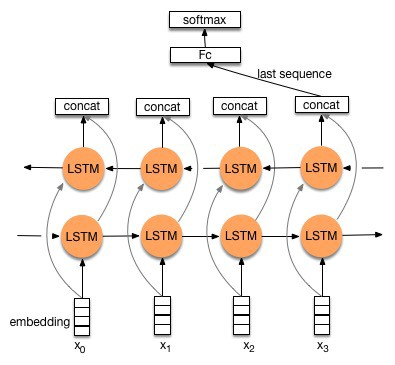
\includegraphics[scale=0.50]{../figs/blstm/diagram.jpeg}	
\caption{BLSTM Architecture}
\label{fig:BLSTM_Arch} 
\end{figure}


\subsection{Convolutional Neural Networks (CNN)}
% Give a little introduction about how CNNs work and why are they use. Show how they were designed to extract local features and how they learn it. This section will cover the basics of convolution, activations like RELU and things like max pooling
For this project we will also be focusing on CNNs. They apply a technique termed as Convolutions, which refer to a weighted sum of values slided over the input to get an output. Convolutions are often referred as Kernels because they are functions/maps/filters which are slided over the input features to get the output features. Because of convolutions CNN's become very powerful because they are automatically able to learn different latent visual features also termed as \textit{"feature maps"}. Considering that CNNs learn these high dimensional feature maps from the given input we aim to use CNNs to extract these features and then build a neural network model on top of these features to classify the audio dataset. A simple CNN architecture often involves multiple layers of several of these convolution layers. Each of these layers are then seperated by a nonlinearity. One of the most commonly used non linearity is \textbf{Rectified Linear Unit (ReLU)} \cite{imagenet_original}. The biggest advantage of ReLU is that the gradient value for ReLU is either $1$ or $0$, hence either the gradient passes just through the convolution or does not, effectively eliminating the problem of vanishing and exploding gradients.

\begin{figure}[!h]
\centering
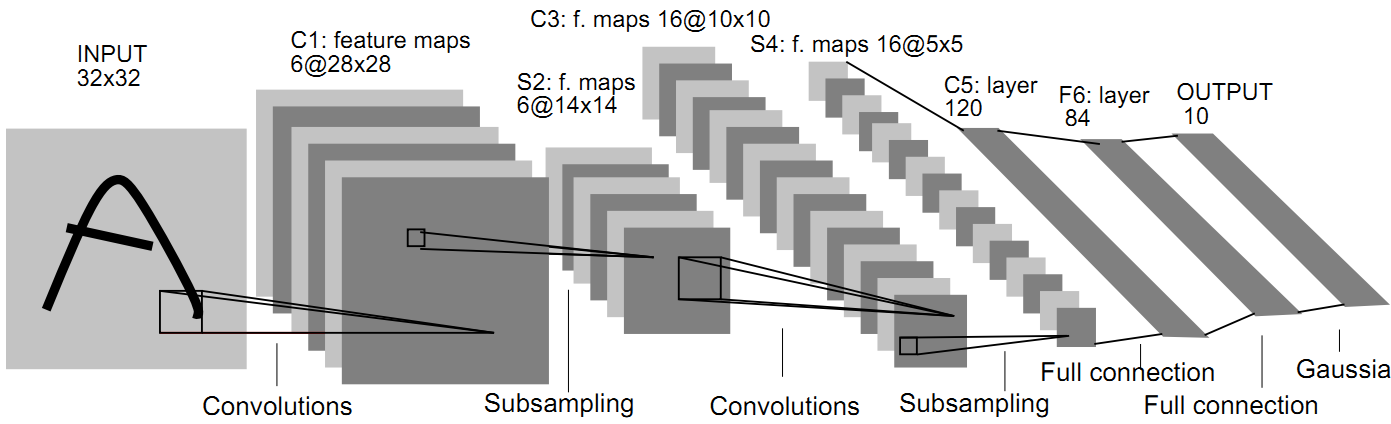
\includegraphics[width=8cm,height=3cm]{../figs/cnn/le_net.png}	
\caption{Le Net \cite{le_net}: One of the earliest successful CNN}
\label{fig:Le_Net_Arch} 
\end{figure}

One of the earliest developed and successful CNNs was developed by Yan Le Cunn \cite{le_net} and trained on the MNIST dataset \ref{fig:Le_Net_Arch}. It was designed to recognise different mathematical digits. This was one of the greatest development in the field of image recognition. After that with the introduction of Imagenet challenge \cite{ilsvrc} and powerful Graphical Processing units, deeper architectures were developed which exceeded human performance. One of the best models was called Resnet-152, containing 152 hidden layers. The architecture for Resnet-152 was distinct from other architectures because of the added residual connections (Figure: \ref{fig:Resnet_Residual_Arch}, which were again added for smoother flow of the gradient through the network.

\begin{figure}[!h]
\centering
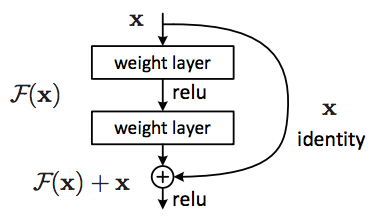
\includegraphics[scale=0.30]{../figs/cnn/resnet_residual.png}	
\caption{Residual Connections in Resnet}
\label{fig:Resnet_Residual_Arch} 
\end{figure}

Because of a lot of stacked convolution layers all the feature maps start learning higher dimensional features which cannot be described beforehand by a human. This is what made it perform exceedingly well. Deeper CNNs are although very powerful but they also become very hard to interpret because as a human it becomes harder to understand what those higher dimensional features represent.

In this project we try to use CNN's for the purpose of exploring how well do they do in processing time dependent data and to understand how well CNNs can learn local features from different images which have been produced by processing an audio signal.

\subsection{Stacking}

Because CNN's are specifically designed to handle at least Two Dimensional data, for the terms of this project there are two ways of converting audio signal data (one dimensional) to an image (two dimensional). The first way is termed as stacking because it just refers to splitting an audio signal data vector into equal sized smaller vectors and stacking them on top of one other, hence the name stacking.

\begin{figure}[!h]
\centering
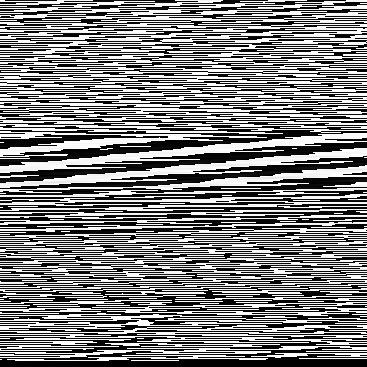
\includegraphics[scale=0.30]{../figs/stacking/sax.jpg}	
\caption{Stacked Image of Saxophone Audio Signal}
\label{fig:Sax_Stack} 
\end{figure}

\subsection{Multiresolution Recurrent Plot (MRP)}

Other than stacking there also exist other techniques to convert audio data signals into an image. One of the techinques we are also considering for this project is called Multiresolution Recurrence Plot (MRP). As mentioned in Park et al. \cite{cnn_music_mrp} using MRPs, time series data can be analyzed in the two dimensional space without losing any information. A traditional recurrent plot is used to measure the distance between two different phase trajectories at all different possible timestep combinations. It helps to visualize how a sequence or trajectory occurs again or repeats, which defines the recurrent pattern. The equation behind RPs is as follows:
\begin{equation}
R[i, j] = |{x[i] - x[j]}|
\end{equation}

RPs are very popular for converting time series data into image based data in the field of mediciene. We can use a similar techinque for the case of the instruments and their recordings. However, because different instruments have very different frequency, it becomes important to use different sized window techinques for each recurrent plot from the same instrument so that all instruments and their respective frequency range can be visualized in the plot. MRPs implement this by actually extracting different size of samples from the same time series data and then constructing a RP on top of them. However because CNNs are fixed in terms of the input size, we use pooling layers to get the same size even for different sized input time series sample. Example of a MRP for Saxophone is below in Figure: \ref{fig:MRP_Sax}.	
\begin{figure}[!h]
\centering
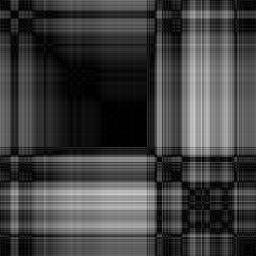
\includegraphics[scale=0.40]{../figs/mrp/sax.jpg}	
\caption{Recurrence Plot for Saxophone}
\label{fig:MRP_Sax} 
\end{figure}

\subsection{CNN \& RNN}
RNNs are very powerful in modelling sequential data, while CNNs are very powerful in extracting features. Models like RCNN \cite{cnn_rnn_sleep_staging} or CRNN \cite{crnn} combine the two types or architecture in a sequential way. They first apply a CNN on a 2-Dimensional representation of the audio data and then connect the output from the CNN layer as the initial hidden state for the RNN architecture (LSTM cell) which is trained over the actual raw audio data.

%Until now, we have talked about how RNNs are a very powerful tool for modelling sequential data because of their innate capabilities of holding memory from past and sometimes even the future data. While on the other hand CNNs are powerful tool for modelling visual data because of their property of learning latent high dimensional features. Considering that our problem works on the concept of Audio Classification/Image recognition such that we already have all the audio data as .wav files and also using the techinque mentioned before about MRP we can also convert our time series data into an image, we are also trying to implement the kind of network used in Aggarwal et al. \cite{cnn_rnn_sleep_staging}
%which combines CNNs and RNNs. The network mentioned in \cite{cnn_rnn_sleep_staging} works well for Sleep staging, however we will change the architecture a little bit to suit our problem. We will apply CNN on the MRP images to learn various latent high dimensional features and pass the information about these features to an LSTM cell as its initial internal state. We will be using LSTM and not GRU, because it can be seen that LSTM cells have been already used in Audio Classification \cite{lstm_music_genre} and performed very well.

%For this project the implementation will all be done in Python. Python is an open source interpreted high-level programming language for general-purpose programming. Currently python supports a lot of powerful libraries like Keras, Tensorflow and Pytorch which provide enough resources to set up different deep learning architectures that have been mentioned before. Along with these libraries there also exist some other libaries like numpy, scipy, sklearn and matplotloib which will help in data loading, preprocessing, analysis and visualizations. All of these libaries have lots of great documentation available online and also a lot of blog articles on websites like Medium and TowardsDataScience containing helpful resources related to the full spectrum. On my initial analysis, there is not much code available online directly corresponding to my problem. I will be coding the chunk of the whole project but most of it will be based off online discussions and blogs where people try to use these architectures for different yet similar problems.

%%%%%%%%%%%%%%%%%%%%%%%%%%%%%%%%%%%%%%%%%%%%%%%%%%%%%%%%%%%%%%%%%%%%%%%%%%%%%%%%
%%%%%%%%%%%%%%%%%%%%%%%%%%%%%%%%%%%%%%%%%%%%%%%%%%%%%%%%%%%%%%%%%%%%%%%%%%%%%%%%



%%%%%%%%%%%%%%%%%%%%%%%%%%%%%%%%%%%%%%%%%%%%%%%%%%%%%%%%%%%%%%%%%%%%%%%%%%%%%%%%
% EXPERIMENT
%%%%%%%%%%%%%%%%%%%%%%%%%%%%%%%%%%%%%%%%%%%%%%%%%%%%%%%%%%%%%%%%%%%%%%%%%%%%%%%%
\section{\textbf{Experiment}}

\subsection{Dataset}

For solving the problem statement, we will be using the Instrument Recognition in Music Audio Signals (IRMAS) Dataset \cite{IRMAS_Dataset}. The IRMAS dataset currently has divided the dataset into Training and Test sets. Training Dataset contains 6705 16 bit stereo wav format audio files sampled at 44.1 kHz. All of these files are 3 second excerpts from more than 2000 distinct recordings. The number of audio files for each given class (for this project) is given in Table \ref{tab:pd}. For the Test Set there are 2874 excerpts in 16 bit stereo wav format sampled at 44.1kHz. Considering that these files are not necessarily 3 seconds long, while all of the training files are just 3 seconds long, we are using a Sliding Window approach to actually predict the class for each test file. The sliding window would create the required interval dataset from the test audio files. 

\subsection{Preprocessing Raw Audio Data}
For our project, because we will not be using the entire 3 second window of the input audio data as one single input record, we first created a training data loader script. The script focuses on preprocessing the raw audio data so that it is of the format which can be used to train a Recurrent Neural Network. The script uses the python's scipy.io module to load the data from each audio file and distributes it into two different arrays corresponding to the different audio channels. Then the script normalizes the data to a range between $[-1, 1]$. After that the script converts the whole array into smaller chunks using a sliding window such that each smaller chunk represents the vector length for the RNN cell at each input timestep, and the number of small chunks from each audio sample file represents the number of timesteps of data. To accomplish all of this, we took advantage of Python's Numpy module for easy reshaping and casting operations on the whole dataset.

\subsection{Audio Data to Stacked Images}
Because we are also building models which use CNNs, we have created scripts which convert the raw audio data into a 2-Dimensional image. For the purpose of this project and because CNN's are well suited to process square images, we first \textit{zero-pad} the audio signal data until the length of the vector becomes a perfect square. After this preprocessing, we just reshape the vector to a matrix with first N elements in the first row, then the second N elements in the second row and so on to get a $N$ x $N$ greyscale image. For accomplishing this task, we used the Python's Numpy module to do array reshaping, while used OpenCV module to save images. Two examples of the images I constructed for this project can be seen in Figure: \ref{fig:Vio_Stack} and Figure: \ref{fig:Voi_Stack}.

\begin{figure}[!htb]
   \begin{minipage}{0.24\textwidth}
     \centering
     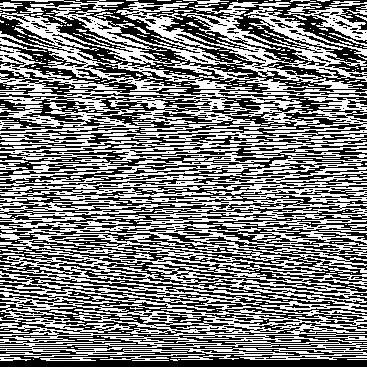
\includegraphics[width=.7\linewidth]{../figs/stacking/vio.jpg}
     \caption{Violin}\label{fig:Vio_Stack}
   \end{minipage}\hfill
   \begin{minipage}{0.24\textwidth}
     \centering
     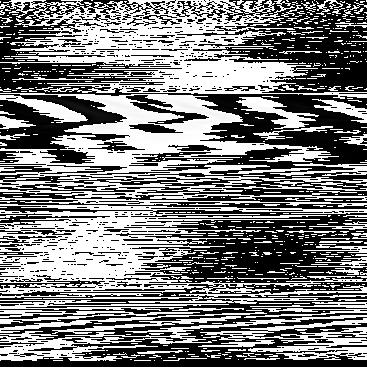
\includegraphics[width=.7\linewidth]{../figs/stacking/voi.jpg}
     \caption{Human Voice}\label{fig:Voi_Stack}
   \end{minipage}
\end{figure}

\subsection{Audio Data to Multiresolution Recurrence Plots}
We also built scripts that use the techniques mentioned in Park et al \cite{cnn_music_mrp} to build our own Multiresolution Recurrence Plots. These scripts load the data from the different audio files and for each audio files pull out different sizes of sliding window data and then use the formula mentioned in Park et al \cite{cnn_music_mrp}. We used python's tensorflow module to execute sliding window, 1-D max pooling, 2-D max pooling operations for faster computation on tensors which were construted from the original data loaded from the audio files. Some examples of the MRP constructed are as follows:

\begin{figure}[!htb]
   \begin{minipage}{0.24\textwidth}
     \centering
     
\includegraphics[width=.7\linewidth]{../figs/mrp/vio.jpg}
     \caption{Violin}\label{fig:Vio_MRP}
   \end{minipage}\hfill
   \begin{minipage}{0.24\textwidth}
     \centering
     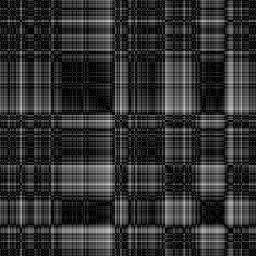
\includegraphics[width=.7\linewidth]{../figs/mrp/voi.jpg}
     \caption{Human Voice}\label{fig:Voi_MRP}
   \end{minipage}
\end{figure}

\subsection{RNN training}
For training the RNN models, we construct different \textbf{ipython notebooks} that import functions from the scripts mentioned before to load the audio data into the memory. Then we use python's Keras module (Deep Learning library) for defining our own RNN architectures with the required parameters. For each notebook we define a new sequential model which contains a type of RNN cell along with fully connected layers at the end. We also add different types of activations and dropout layers in between to avoid overfitting. Then we use tensorflow's tensorboard utility to monitor the training of our models. We also use checkpoints on validation loss and early stopping criteria to avoid wasting processing power on many epochs of training. To test our model, we use the sklearn library to split our training data into train and test dataset and evaluate our model on the test set.

\subsection{CNN training}
For training the CNN models, we construct different \textbf{ipython notebooks} that define generator functions for the training using the Keras library. These generator functions point to the directories containing the various stacking/mrp images already developed using the mentioned scripts. After that we use Keras module for defining our own CNN architectures with different convolutional layers, with the required parameters. For each notebook we define a new sequential model which contains different number of CNN layers along with fully connected layers at the end. We also add \textbf{ReLU} activations among the convolution blocks, while \textbf{Softmax} activation for the final classification layer and dropout layers in between to avoid overfitting. Then we use tensorflow's tensorboard utility to monitor the training of our models. We also use checkpoints on validation loss and early stopping criteria to avoid wasting processing power on many epochs of training. To test our model, evaluate our model on a seperate held out test set.
%For this project I will be setting up different experiments in different notebooks that will walkthrough what type of experiment is being conducted along with the final assessment of that experiment. Most of the experiments would correspond to using different architectures with the same input dataset and similar values of the hyperparameters. For this part of the experiment, I would first compare all the 4 types of RNN's for some binary classification and then compare them on the multiclass comparison containing all the classes that I am considering. Similarly I would also experiment with the two types of CNN models discussed earlier with binary and multiclass classification. These experiments would lead to analysis based on using different architectures for the same dataset over the type of classification being performed. The other type of experiments that I will be performing includes experimenting with the data preprocessing which includes different types of normalization (mean normalization, variance normalization, uniform normalization) on the data and also experimenting with windowing techniques which would deal with the amount of data being loaded. I am especially considered with windowing because it would highly affect the amount of data on which I will be training and also the values of the audio signal I will be using. I am planning to experiment with different sliding window sizes to get a better understanding of the effect of the initial dataset size on the classification accuracy of the model. Other than these I will also do some experimentation to understand the effect of hyperparameters of the architectures on their performance. These experiments however would be each architecture specific. For hyperparameters I will be experimenting with different activation functions, dropout percentages, number and size of layers.

%%%%%%%%%%%%%%%%%%%%%%%%%%%%%%%%%%%%%%%%%%%%%%%%%%%%%%%%%%%%%%%%%%%%%%%%%%%%%%%%
%%%%%%%%%%%%%%%%%%%%%%%%%%%%%%%%%%%%%%%%%%%%%%%%%%%%%%%%%%%%%%%%%%%%%%%%%%%%%%%%





%%%%%%%%%%%%%%%%%%%%%%%%%%%%%%%%%%%%%%%%%%%%%%%%%%%%%%%%%%%%%%%%%%%%%%%%%%%%%%%%
% RESULTS
%%%%%%%%%%%%%%%%%%%%%%%%%%%%%%%%%%%%%%%%%%%%%%%%%%%%%%%%%%%%%%%%%%%%%%%%%%%%%%%%
\section{\textbf{Results}}
For this section, results of each type of model architecture are presented in the order they were discussed. For each type of model different architectures (different number of layers, size of layers, activation functions) were used and were trained on the same training set and validation set. Their performance was recorded on the same test set and is listed here. For this project, we are just focusing on \textit{Accuraccy} of the model as the evaluation factor. In our results section we have mentioned all the three accuraccy metrics (Training, Validation and Testing) so that an easy comparision can be made. 

\subsection{\textbf{Recurrent Neural Networks}}
For all the Recurrent Neural Network based model, we experimented with the number of hidden units ($H$) present in the cell for the type of model used. Other than that because Recurrent Neural Network expect a certain length input at every timestep, we also experimented with the size of the input vector ($|X_t|$) at each timestep for the models. This was equivalent to changing the number of timesteps of data present. For our dataset the total length of the feature vector was constant for each training sample, hence we divided the feature vector into multiple equal size vectors using a sliding window approach to represent the input vector for the corresponding timestamp, which is why changing the size of the input vector length also changes the number of timesteps.

\subsubsection{Vanilla RNN Model}
For the Vanilla RNN model, our base model was a RNN cell along with a Dropout layer (to avoid overfitting) connected to a Dense Layer used as a classification layer with the help of softmax activation function for multiclass classification. The architecture for the base model is depicted in Appendix B, Figure: \ref{fig:Vanilla_RNN_Arch_Model}. 

Results are mentioned in Table \ref{tab:RNN_Acc}

\begin{table}[!h]
\centering
\caption{Vanilla RNN Model Results}
\begin{tabular}{| c || c || c || c || c |} %sets the format of the table
\hline %horizontal line
 $|X_t|$ & $H$ & Train Acc & Validation Acc & Test Acc\\
   \hline \hline
300 & 50 & 0.512 & 0.481 & 0.3713 \\
\hline
300 & 100 & 0.563 & 0.504 & 0.4952 \\
\hline
300 & 150 & 0.587 & 0.522 & 0.489 \\	
\hline
100 & 50 & 0.307 & 0.271 & 0.157 \\
\hline
100 & 100 & 0.336 & 0.295 & 0.186 \\
\hline
100 & 150 & 0.319 & 0.242 & 0.164 \\
\hline
   \end{tabular}
\label{tab:RNN_Acc} 
\end{table}


\subsubsection{LSTM Model}
For the LSTM model, our base model was a LSTM cell along with a Dropout layer (to avoid overfitting) connected to a Dense Layer used as a classification layer with the help of softmax activation function for multiclass classification. For the case of LSTM because the model had much more number of parameters we increased the number of epochs for which it was being trained. The architecture for the base model is depicted in Appendix B, Figure: \ref{fig:LSTM_Arch_Model}

Results are mentioned in Table \ref{tab:LSTM_Acc}

\begin{table}[!h]
\centering
\caption{LSTM Model Results}
\begin{tabular}{| c || c || c || c || c |} %sets the format of the table
\hline %horizontal line
 $|X_t|$ & $H$ & Train Acc & Validation Acc & Test Acc\\
   \hline \hline
300 & 50 & 0.640 & 0.6714 & 0.653 \\
\hline
300 & 100 & 0.673 & 0.6509 & 0.6817 \\
\hline
300 & 150 & 0.662 & 0.6212 & 0.6393 \\	
\hline
100 & 50 & 0.726 & 0.6948 & 0.7184 \\
\hline
100 & 100 & 0.783 & 0.7614 & 0.7538 \\
\hline
100 & 150 & 0.769 & 0.752 & 0.7441 \\
\hline
   \end{tabular}
\label{tab:LSTM_Acc} 
\end{table}


\subsubsection{GRU Model}
For the GRU model, our base model was a GRU cell along with a Dropout layer (to avoid overfitting) connected to a Dense Layer used as a classification layer with the help of softmax activation function for multiclass classification. The architecture for the base model is depicted in Appendix B, Figure: \ref{fig:GRU_Arch_Model}

Results are mentioned in Table \ref{tab:GRU_Acc}

\begin{table}[!h]
\centering
\caption{GRU Model Results}
\begin{tabular}{| c || c || c || c || c |} %sets the format of the table
\hline %horizontal line
 $|X_t|$ & $H$ & Train Acc & Validation Acc & Test Acc\\
   \hline \hline
300 & 50 & 0.617 & 0.6003 & 0.600 \\
\hline
300 & 100 & 0.668 & 0.6525 & 0.632 \\
\hline
300 & 150 & 0.694 & 0.6427 & 0.633 \\	
\hline
100 & 50 & 0.7012 & 0.675 & 0.638 \\
\hline
100 & 100 & 0.747 & 0.7683 & 0.712 \\
\hline
100 & 150 & 0.7484 & 0.741 & 0.725 \\
\hline
   \end{tabular}
\label{tab:GRU_Acc} 
\end{table}


\subsubsection{BLSTM Model}
For the BLSTM model, our base model was a BLSTM cell along with a Dropout layer (to avoid overfitting) connected to a Dense Layer which is connected to only the last timestamps hidden nodes of the BLSTM cell, used as a classification layer with the help of softmax activation function for multiclass classification. For the case of BLSTM cell, there were more options regarding using the hidden units from each timestamp to connect to the Dense layer. However because of the limited resources on the system, it became harder to train that model and was not considered. The architecture for the base model is depicted in Appendix B, Figure: \ref{fig:BLSTM_Arch_Model}

Results are mentioned in Table \ref{tab:BLSTM_Acc}

\begin{table}[!h]
\centering
\caption{BLSTM Model Results}
\begin{tabular}{| c || c || c || c || c |} %sets the format of the table
\hline %horizontal line
 $|X_t|$ & $H$ & Train Acc & Validation Acc & Test Acc\\
   \hline \hline
300 & 50 & 0.583 & 0.549 & 0.5218 \\
\hline
300 & 100 & 0.5914 & 0.571 & 0.5336 \\
\hline
300 & 150 & 0.589 & 0.585 & 0.5461 \\	
\hline
100 & 50 & 0.642 & 0.5978 & 0.55 \\
\hline
100 & 100 & 0.657 & 0.6614 & 0.5809 \\
\hline
100 & 150 & 0.655 & 0.6329 & 0.6216 \\
\hline
   \end{tabular}
\label{tab:BLSTM_Acc} 
\end{table}


As we can observe that for each model the accuracy on the test set is not really high. So we think this was because of using just one Dense layer directly as the classification layer from the hidden units of the different models. We then experimented by adding another Dense layer inbetween such that it contained around 50 nodes, and it was then connected to the classification dense layer. For the new Dense layer we used the ReLU activation function as the nonlinearity for better gradient flow. The results of the experiments for one particular parameter for each of the RNN type model are depicted as in Table \ref{tab:2Dense}.

\begin{table}[!h]
\centering
\caption{All Models with Added Dense Layer}
\begin{tabular}{| c || c || c || c |} %sets the format of the table
\hline %horizontal line
Model & $|X_t|$ & $H$ & Test Acc\\
   \hline \hline
Vanilla RNN & 300 & 50 & 0.4516\\
\hline
LSTM & 300 & 50 & 0.7063\\
\hline
GRU & 300 & 50 & 0.7134\\	
\hline
BLSTM & 300 & 50 & 0.5579  \\
\hline
   \end{tabular}
\label{tab:2Dense} 
\end{table}


\subsection{\textbf{Convolutional Neural Networks}}
For this section, results of each type of images on which the simple Convolutional Neural Networks were implemented are presented in the order they were discussed. For each type of image, we defined our own Convolutional Neural Network including different convolutional layers, maxpooling layers and finally dense layers. For this section of the project, we experimented with the size of the convolutional filters in each model along with the size of the Max Pooling operations and strides of each of these layers. For each model we primarily used \textit{ReLU} activation function. All the models were trained on the same training set and validation set image generators. Their performance was recorded on the same test set generator and is listed here. For this project, we are just focusing on \textit{Accuraccy} of the model as the evaluation factor. In our results section we have mentioned all the three accuraccy metrics (Training, Validation and Testing) so that an easy comparision can be made. We used the \textit{.jpg} format to save all the images. We used our own defined generator functions with the help of Keras that just normalizes the image data to load the images. All the images were resized to a smaller size to decrease the overall number of parameters and also the depth of the model architecture. Different models that we constructed are mentioned in Appendix B.

\subsubsection{Stacking Images}
Results are mentioned in Table \ref{tab:Stacking_Acc}
\begin{table}[!h]
\centering
\caption{CNN performance on Stacking Images}
\begin{tabular}{| c || c || c || c |} %sets the format of the table
\hline %horizontal line
Model & Training Acc & Validation Acc & Test Acc\\
   \hline \hline
B1 & 0.5034 & 0.4819 & 0.4771 \\
\hline
B2 & 0.5412 & 0.5193 & 0.5076 \\
\hline
B3 & 0.5683 & 0.5546 & 0.5453 \\	
\hline
B4 & 0.5885 & 0.502 & 0.4683  \\
\hline
   \end{tabular}
\label{tab:Stacking_Acc} 
\end{table}



\subsubsection{Multiresolution Recurrence Plot}
Results are mentioned in Table \ref{tab:MLP_Acc}
\begin{table}[!h]
\centering
\caption{CNN performance on MLP Images}
\begin{tabular}{| c || c || c || c |} %sets the format of the table
\hline %horizontal line
Model & Training Acc & Validation Acc & Test Acc\\
   \hline \hline
B1 & 0.6532 & 0.633 & 0.6053 \\
\hline
B2 & 0.6779 & 0.6841 & 0.6785 \\
\hline
B3 & 0.7412 & 0.7319 & 0.7104 \\	
\hline
B4 & 0.7943 & 0.6021 & 0.5307  \\
\hline
   \end{tabular}
\label{tab:MLP_Acc} 
\end{table}


\subsubsection{RCNN or CRNN}
For this project, I was not able to train the CRNN model for enough epochs as it proved to be very difficult for me to set it up in a timely manner. Even after I was able to set it up, it included a lot of parameters and because of no access to a GPU (Graphical Processing Unit) it became hard to train the model on my machine with only CPU. Each epoch was taking around 16 minutes to complete. Also as I was not able to use a generator function, it was very internsive on the memory which also contributed to such slow training. I tried to using Google Collaboratory, however loading all the data into the memory seemed to exceed the resources allocated and thus was not able to use it.  The results of training different RCNN models with the base CNN models as mentioned in Appendix B, along with a LSTM cell after training for just 10 epochs is in Table \ref{tab:CRNN_Acc}

\begin{table}[!h]
\centering
\caption{RCNN or CRNN performance on MLP Images}
\begin{tabular}{| c || c || c || c |} %sets the format of the table
\hline %horizontal line
Model & Training Acc & Validation Acc & Test Acc\\
   \hline \hline
B1 & 0.5075 & 0.4938 & 0.4017 \\
\hline
B2 & 0.5314 & 0.4873 & 0.4822 \\
\hline
B3 & 0.5753 & 0.5579 & 0.5410 \\	
\hline
B4 & 0.5642 & 0.5348 & 0.4806  \\
\hline
   \end{tabular}
\label{tab:CRNN_Acc} 
\end{table}

%%%%%%%%%%%%%%%%%%%%%%%%%%%%%%%%%%%%%%%%%%%%%%%%%%%%%%%%%%%%%%%%%%%%%%%%%%%%%%%%
%%%%%%%%%%%%%%%%%%%%%%%%%%%%%%%%%%%%%%%%%%%%%%%%%%%%%%%%%%%%%%%%%%%%%%%%%%%%%%%%



%%%%%%%%%%%%%%%%%%%%%%%%%%%%%%%%%%%%%%%%%%%%%%%%%%%%%%%%%%%%%%%%%%%%%%%%%%%%%%%%
% ANALYSIS
%%%%%%%%%%%%%%%%%%%%%%%%%%%%%%%%%%%%%%%%%%%%%%%%%%%%%%%%%%%%%%%%%%%%%%%%%%%%%%%%
\section{\textbf{Analysis}}

\subsection{\textbf{Recurrent Neural Networks}}
In all the different types of RNN models that we experimented with, we can easily infer that the models that performed worst was Vanilla RNN model. This model has consistently low accuracies  with some of them under the random agent baseline (20\%). This was expected because Vanilla RNN models do not perform well on modelling sequence because of the problem of Vanishing Gradients \cite{vanishing_gradient}. Also, as mentioned earlier Vanilla RNN's performance degrades with longer sequences, we can easily observe that fact when we decrease the size of the input vector, thus essentially increasing the number of timestamps in each series (tripling it). In this case Vanilla RNN's perform worse than a random agent on the test set and seems to indicate that it had overfit part of the dataset and then stopped updating the gradients because of the problem of Vanishing Gradients \cite{vanishing_gradient}. However when we observer other models we see that their overall accuracy on the given test set is not as high as expected, however they are pretty decent classifiers and have actually learned something.

All the models Vanilla RNN, LSTM, GRU and BLSTM show that with the increase in size of the number of hidden units in the cell there was an increase in the overall accuracies. However if we observer carefully, we can see that with very large number of hidden units the model essentially starts to overfiit, as can be seen in cases where the accuracy for 150 hidden units is a little less than that of 100 hidden units. Other than this fact we can also observe that models like LSTM and GRU shows a trend, where they perform better on sequences which are longer. According to Table \ref{tab:LSTM_Acc} and Table \ref{tab:GRU_Acc}, LSTM and GRU performs better when the input vector size is decreased (increased length of the sequence). This result was a little bit unexpected because the length of the sequence was almost tripled (input vector size was divided by 3) which results in a very long sequence. However this result demonstrates the strength of LSTM and GRU models. Using intricate dependencies and allowing for smoother gradient flow helps these models to surpass the performance of the simple Vanilla RNN models.

Among LSTM and GRU, for our case LSTM performed better most of the times, however the difference was not really that significant. Most of the times the difference in accuracy was within 4 units. It is important to note that during our training process we ran LSTM training for a little longer so that the model can converge appropriately. We suspect this might be the case that GRU just sometimes gets left behind. Other interesting thing we notice is that the BLSTM model that we trained didnt really perform as good as its LSTM and GRU counterparts. This result was a little bit astonishing because BLSTM models just more contextual information from past and future. We suspect that the reason BLSTM performs worse than both LSTM and GRU models is because in music signals there are no context dependencies like there are in English language. Music signals are not vague, and inherently are always recorded in one direction as there is no way to go back in time. We think the fundamental assumption in BLSTM models that current timestamp values are affected by both past and future values was very much different from the way music signals behave and thus did not perform as well.

One of the more interesting observations that we can make from the Recurrent Neural Networks result section is that no model performed exceedingly well. This was because we were just using one Dense layer to do classification. It is always advised to combine some dense layers to form a fully connected network before doing classification so that the network can still learn some more high dimensional features. Hence when we take a look at Table \ref{tab:2Dense}, we see that most of the models improved their test accuracies by the addition of the Dense layers.


\subsection{\textbf{Convolutional Neural Networks}}
When we start comparing different CNN models we observe that CNNs performed better on images of the Multiple Recurrence Plots than on images constructed using Stacking. It was very interesting to find that there was a noticeable difference between the accuracies of the models for both types of images. Upon further inspection for the cause of the difference, I found out that the models built on stacking images usually had very similar probabilities for different classes like Electric Guitar, Piano and Human Voice had similar probabilities and Saxophone and Violin also had very similar probabilities in the classification layer after the softmax activation. This was an indicator of bad training data. After observing this, I started looking at different images for each of the classes and found that most of the images in Saxophone and Violin class were infact very similar. A lot of the images usually were similar in terms of having one big strip depicting overtones and all other parts of images just some garbled up combination of black and white. One example that I found was for images in Figures \ref{fig:Vio_sim_stacking}, \ref{fig:Sax_sim_stacking}.

\begin{figure}[!htb]
   \begin{minipage}{0.24\textwidth}
     \centering
     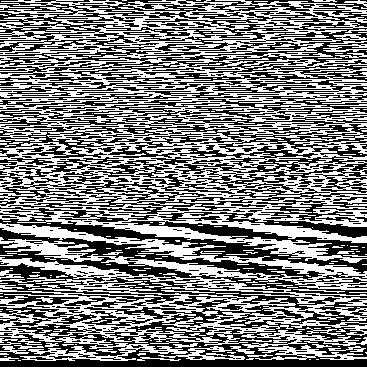
\includegraphics[width=.7\linewidth]{../figs/similar_stacking/vio.jpg}
     \caption{Violin}\label{fig:Vio_sim_stacking}
   \end{minipage}\hfill
   \begin{minipage}{0.24\textwidth}
     \centering
     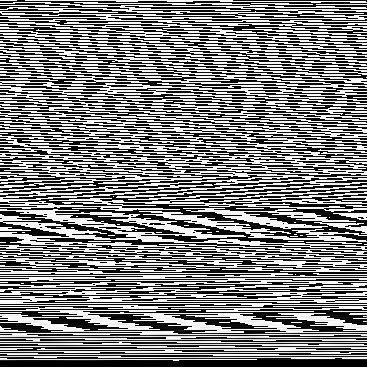
\includegraphics[width=.7\linewidth]{../figs/similar_stacking/sax.jpg}
     \caption{Saxophone}\label{fig:Sax_sim_stacking}
   \end{minipage}
\end{figure}


Other than this one observation that we can make is that Model 3 performs better than the other models. This could be because of the fact that this model was a little more deeper, had an extra convolutional layer which helped it learn more abstract features and thus performed a little better than other models. Also we see that model 2 performed better than model 1 because it had less strides and had more parameters to learn because of more convolution filters and smaller max pooling and convolution filter size. One interesting observation is that model 4 performs worse than model 3 even though it has more convolution layers than it. We suspect that the reason for this is because we are not using an max pooling layers which might lead to overfitting.

For this project, we were not able to train the CRNN models for enough number of epochs. However they still performed pretty well, which depicts that stacking different types of deep learning models on each other such that they can extract features and also model the time series could be very powerful.
%%%%%%%%%%%%%%%%%%%%%%%%%%%%%%%%%%%%%%%%%%%%%%%%%%%%%%%%%%%%%%%%%%%%%%%%%%%%%%%%
%%%%%%%%%%%%%%%%%%%%%%%%%%%%%%%%%%%%%%%%%%%%%%%%%%%%%%%%%%%%%%%%%%%%%%%%%%%%%%%%



%%%%%%%%%%%%%%%%%%%%%%%%%%%%%%%%%%%%%%%%%%%%%%%%%%%%%%%%%%%%%%%%%%%%%%%%%%%%%%%%
% CONCLUSION
%%%%%%%%%%%%%%%%%%%%%%%%%%%%%%%%%%%%%%%%%%%%%%%%%%%%%%%%%%%%%%%%%%%%%%%%%%%%%%%%
\section{\textbf{Conclusion and Future Work}}
From this project, we can conclude that using different Deep learning architectures like Recurrent Neural Networks and Convolutional Neural Networks, we can effectively process audio signals without actually preprocessing the data or doing feature extraction. One of the biggest strengths of each of the method described is that they operate on the raw data and learn these features. Because of this, we can assert that using different deep learning based models can help us achieve good performance at the task of Instrument recognition. Also, we can conclude that it is very important to choose the right type of model for the task. Using Vanilla RNN or BLSTM did not work as expected because of the fundamental differences in the structure of data and their assumptions. Considering that audio signals are very long sequences it is always advised to use a LSTM or GRU approach. Other than that we can also conclude that it is very important to validate the training data and also the theory behind the method used to create the training data. As we observed in our case, the technique of Stacking did not really have any theoretical background and also lead to a lot of similar training data, which is why the model did not perform as expected. However CNNs on images of Multresolution Recurrence Plots performed much better because these images have a mathematical theory behind it which is what helps in effective feature extraction. Other than that it is also very important to consider the overall architecture of the fully connected layers at the end which are used for Classification. It is advised to use more than one fully connected layer so that the learned representations can be effectively utilized for classification by inserting non linearities in between and learning new features which are helpful in classification.

This project was just the tip of the iceberg when it comes to using deep learning architectures for the problem of instrument recognition. We only surveyed the different models with just some fundamental differences in the architecture. Future work for this project would include actually using multile cells of the Recurrent Neural Networks stacked on top of each other to create further deep models. Also it would include a more through experimentation of number of fully connected layers, different activation functions, input vector sizes, number of convolutional layers, size of the feature maps etc. Also it would be worthwile to actually experiment with different hyperparameters like Learning Rate, Optimization method, different error metrics. Also for this project because of the lack of hardware and resources we did not train the models for a large number of iterations and on huge amounts of data. It would be advised to collect dedicated music signals from each type of instrument to construct a big Audio library and then use a GPU based machine for training the models for very more epochs.
%%%%%%%%%%%%%%%%%%%%%%%%%%%%%%%%%%%%%%%%%%%%%%%%%%%%%%%%%%%%%%%%%%%%%%%%%%%%%%%%
%%%%%%%%%%%%%%%%%%%%%%%%%%%%%%%%%%%%%%%%%%%%%%%%%%%%%%%%%%%%%%%%%%%%%%%%%%%%%%%%




\begin{thebibliography}{99}

\bibitem{IRMAS_Dataset} Bosch, Juan J., et al. "A Comparison of Sound Segregation Techniques for Predominant Instrument Recognition in Musical Audio Signals." ISMIR. 2012.

\bibitem{google_accoustics} Sak, Haşim, Andrew Senior, and Françoise Beaufays. "Long short-term memory recurrent neural network architectures for large scale acoustic modeling." Fifteenth annual conference of the international speech communication association. 2014.

\bibitem{google_speech} Sak, Haşim, Andrew Senior, and Françoise Beaufays. "Long short-term memory based recurrent neural network architectures for large vocabulary speech recognition." arXiv preprint arXiv:1402.1128 (2014).

\bibitem{imagenet_original} Krizhevsky, Alex, Ilya Sutskever, and Geoffrey E. Hinton. "Imagenet classification with deep convolutional neural networks." Advances in neural information processing systems. 2012.

\bibitem{bidirectional_lstm_speech} Graves, Alex, and Navdeep Jaitly. "Towards end-to-end speech recognition with recurrent neural networks." International Conference on Machine Learning. 2014.

\bibitem{renet} Visin, Francesco, et al. "Renet: A recurrent neural network based alternative to convolutional networks." arXiv preprint arXiv:1505.00393 (2015).

\bibitem{gru_evaluation} Chung, Junyoung, et al. "Empirical evaluation of gated recurrent neural networks on sequence modeling." arXiv preprint arXiv:1412.3555 (2014).

\bibitem{gru_translation} Cho, Kyunghyun, et al. "On the properties of neural machine translation: Encoder-decoder approaches." arXiv preprint arXiv:1409.1259 (2014).

\bibitem{lstm_sequence_modelling} Graves, Alex. "Generating sequences with recurrent neural networks." arXiv preprint arXiv:1308.0850 (2013).

\bibitem{cnn_rnn_sleep_staging} Aggarwal, Karan, et al. "A Structured Learning Approach with Neural Conditional Random Fields for Sleep Staging."

\bibitem{cnn_music_mrp} Park, Taejin, and Taejin Lee. "Musical instrument sound classification with deep convolutional neural network using feature fusion approach." arXiv preprint arXiv:1512.07370 (2015).

\bibitem{lstm_music_genre} Tang, Chun Pui, et al. "Music Genre classification using a hierarchical Long Short Term Memory (LSTM) model." (2018).

\bibitem{vanishing_gradient} Pascanu, Razvan, Tomas Mikolov, and Yoshua Bengio. "On The Difficulty Of Training Recurrent Neural Networks." Arxiv.org. N. p., 2012. Web. 13 Dec. 2018.

\bibitem{lstm_intro} Hochreiter, Sepp, and Jürgen Schmidhuber. "Long short-term memory." Neural computation 9.8 (1997): 1735-1780.

\bibitem{blstm_intro} Yu, Zhou, et al. "Using bidirectional LSTM recurrent neural networks to learn high-level abstractions of sequential features for automated scoring of non-native spontaneous speech." Automatic Speech Recognition and Understanding (ASRU), 2015 IEEE Workshop on. IEEE, 2015.

\bibitem{blstm_protein} Thireou, Trias, and Martin Reczko. "Bidirectional long short-term memory networks for predicting the subcellular localization of eukaryotic proteins." IEEE/ACM Transactions on Computational Biology and Bioinformatics (TCBB) 4.3 (2007): 441-446.

\bibitem{ilsvrc} Olga Russakovsky*, Jia Deng*, Hao Su, Jonathan Krause, Sanjeev Satheesh, Sean Ma, Zhiheng Huang, Andrej Karpathy, Aditya Khosla, Michael Bernstein, Alexander C. Berg and Li Fei-Fei. (* = equal contribution) ImageNet Large Scale Visual Recognition 

\bibitem{le_net} Y. LeCun, L. Bottou, Y. Bengio, and P. Haffner. Gradient-based learning applied to document recognition. Proceedings of the IEEE, november 1998

\bibitem{crnn} Choi, Keunwoo, et al. "Convolutional recurrent neural networks for music classification." 2017 IEEE International Conference on Acoustics, Speech and Signal Processing (ICASSP). IEEE, 2017.

\bibitem{audio_classification} Herrera-Boyer, Perfecto, Anssi Klapuri, and Manuel Davy. "Automatic classification of pitched musical instrument sounds." Signal processing methods for music transcription. Springer, Boston, MA, 2006. 163-200.

\end{thebibliography}










%%%%%%%%%%%%%%%%%%%%%%%%%%%%%%%%%%%%%%%%%%%%%%%%%%%%%%%%%%%%%%%%%%%%%%%%%%%%%%%%
% CNN Model Architectures
%%%%%%%%%%%%%%%%%%%%%%%%%%%%%%%%%%%%%%%%%%%%%%%%%%%%%%%%%%%%%%%%%%%%%%%%%%%%%%%%
\section{\textbf{Appendix A: Code}}
The code for this project is hosted on a \textbf{Github Repository} at location: \href{https://github.com/goelsaksham/organphile}{https://github.com/goelsaksham/organphile}
%%%%%%%%%%%%%%%%%%%%%%%%%%%%%%%%%%%%%%%%%%%%%%%%%%%%%%%%%%%%%%%%%%%%%%%%%%%%%%%%
%%%%%%%%%%%%%%%%%%%%%%%%%%%%%%%%%%%%%%%%%%%%%%%%%%%%%%%%%%%%%%%%%%%%%%%%%%%%%%%%



%%%%%%%%%%%%%%%%%%%%%%%%%%%%%%%%%%%%%%%%%%%%%%%%%%%%%%%%%%%%%%%%%%%%%%%%%%%%%%%%
% RNN Model Architectures
%%%%%%%%%%%%%%%%%%%%%%%%%%%%%%%%%%%%%%%%%%%%%%%%%%%%%%%%%%%%%%%%%%%%%%%%%%%%%%%%
\section{\textbf{Appendix B: All Model Architectures}}

\begin{figure}[!h]
\centering
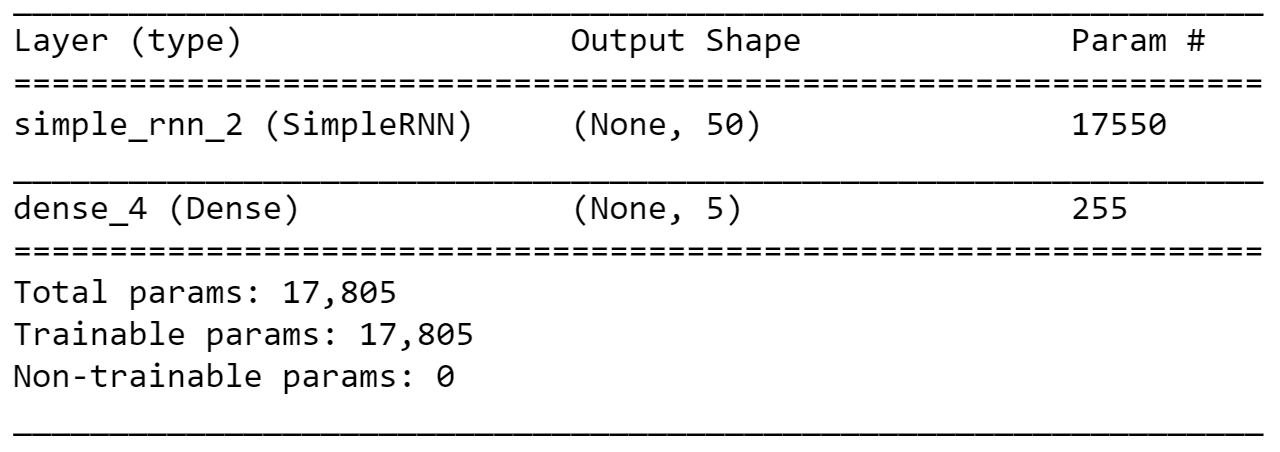
\includegraphics[scale=0.60]{../figs/model_arch/rnn.png}	
\caption{Vanilla RNN Model Sample Architecture}
\label{fig:Vanilla_RNN_Arch_Model} 
\end{figure}

\begin{figure}[!h]
\centering
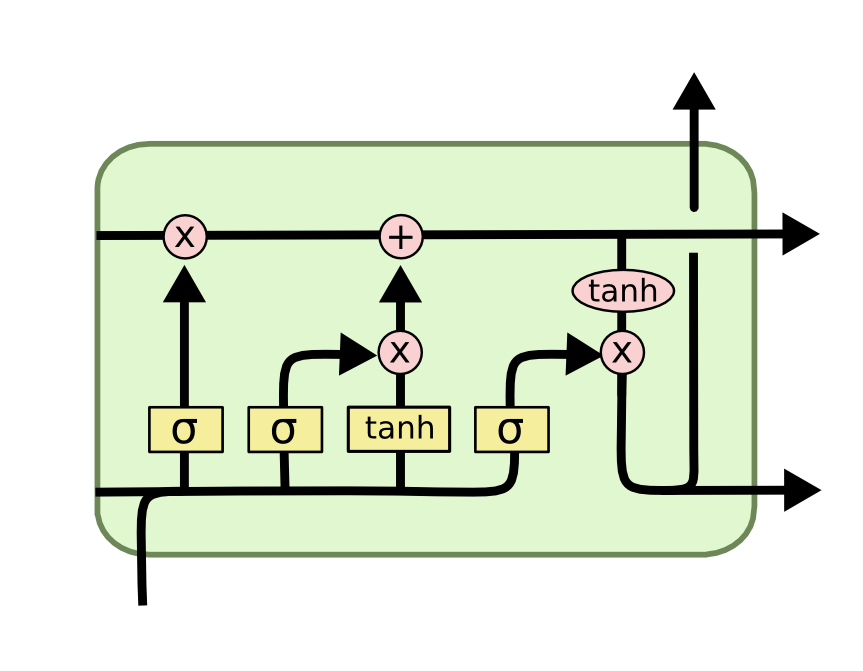
\includegraphics[scale=0.60]{../figs/model_arch/lstm.png}	
\caption{LSTM Model Sample Architecture}
\label{fig:LSTM_Arch_Model} 
\end{figure}

\begin{figure}[!h]
\centering
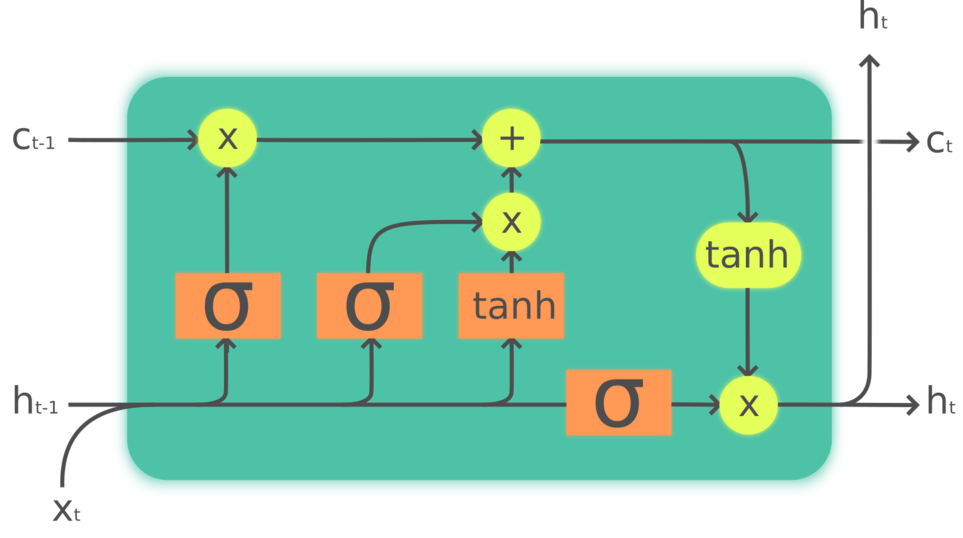
\includegraphics[scale=0.60]{../figs/model_arch/gru.png}	
\caption{GRU Model Sample Architecture}
\label{fig:GRU_Arch_Model} 
\end{figure}


\begin{figure}[!h]
\centering
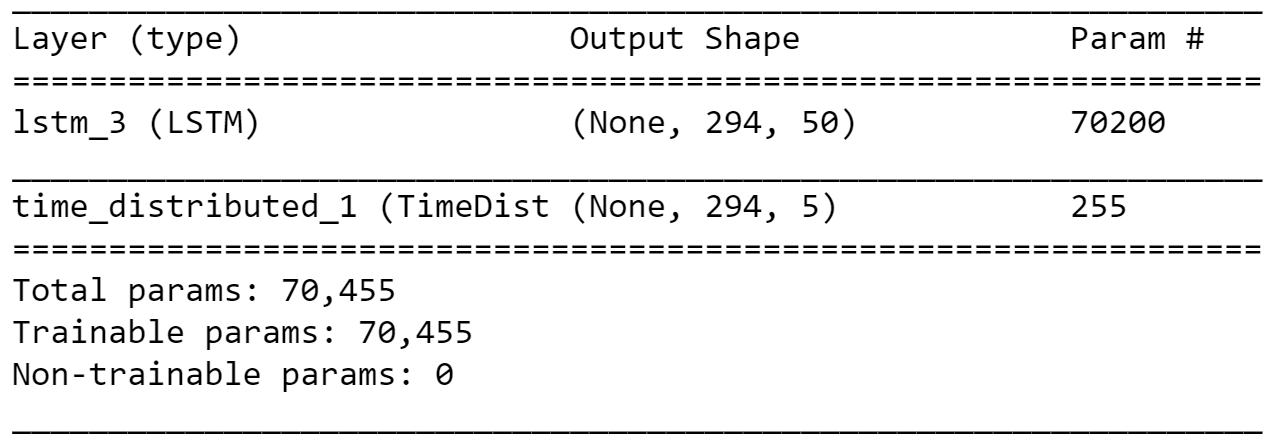
\includegraphics[scale=0.60]{../figs/model_arch/blstm.png}	
\caption{BLSTM Model Sample Architecture}
\label{fig:BLSTM_Arch_Model} 
\end{figure}

%%%%%%%%%%%%%%%%%%%%%%%%%%%%%%%%%%%%%%%%%%%%%%%%%%%%%%%%%%%%%%%%%%%%%%%%%%%%%%%%
%%%%%%%%%%%%%%%%%%%%%%%%%%%%%%%%%%%%%%%%%%%%%%%%%%%%%%%%%%%%%%%%%%%%%%%%%%%%%%%%


%%%%%%%%%%%%%%%%%%%%%%%%%%%%%%%%%%%%%%%%%%%%%%%%%%%%%%%%%%%%%%%%%%%%%%%%%%%%%%%%
% CNN Model Architectures
%%%%%%%%%%%%%%%%%%%%%%%%%%%%%%%%%%%%%%%%%%%%%%%%%%%%%%%%%%%%%%%%%%%%%%%%%%%%%%%%
%\section{\textbf{Appendix C: CNN Model Architectures}}

%This part of the project depicts all the architectures we used for the CNN part of the project.

\begin{figure}[!h]
\centering
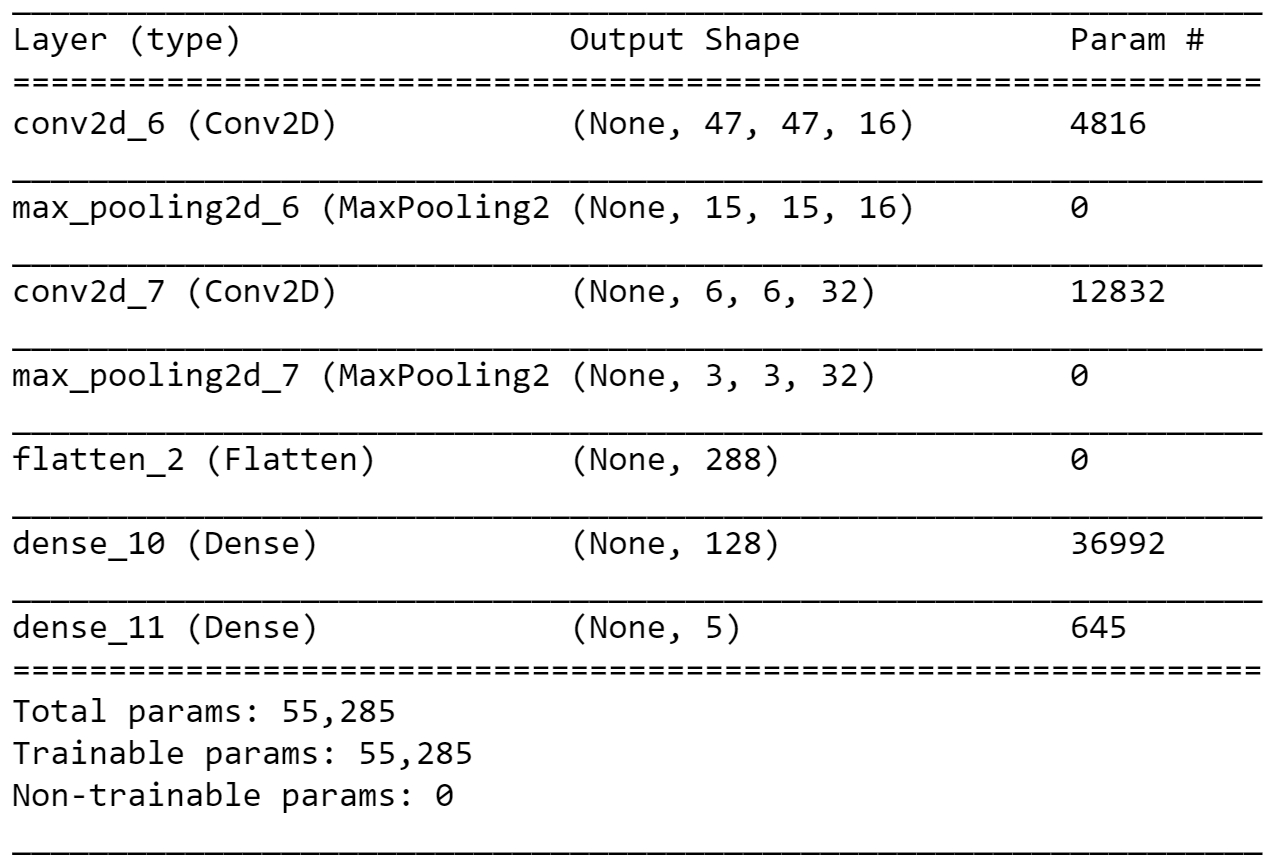
\includegraphics[scale=0.60]{../figs/model_arch/cnn_b1.png}	
\caption{CNN Model B1 Sample Architecture}
\label{fig:CNN_B1_Arch_Model} 
\end{figure}

\begin{figure}[!h]
\centering
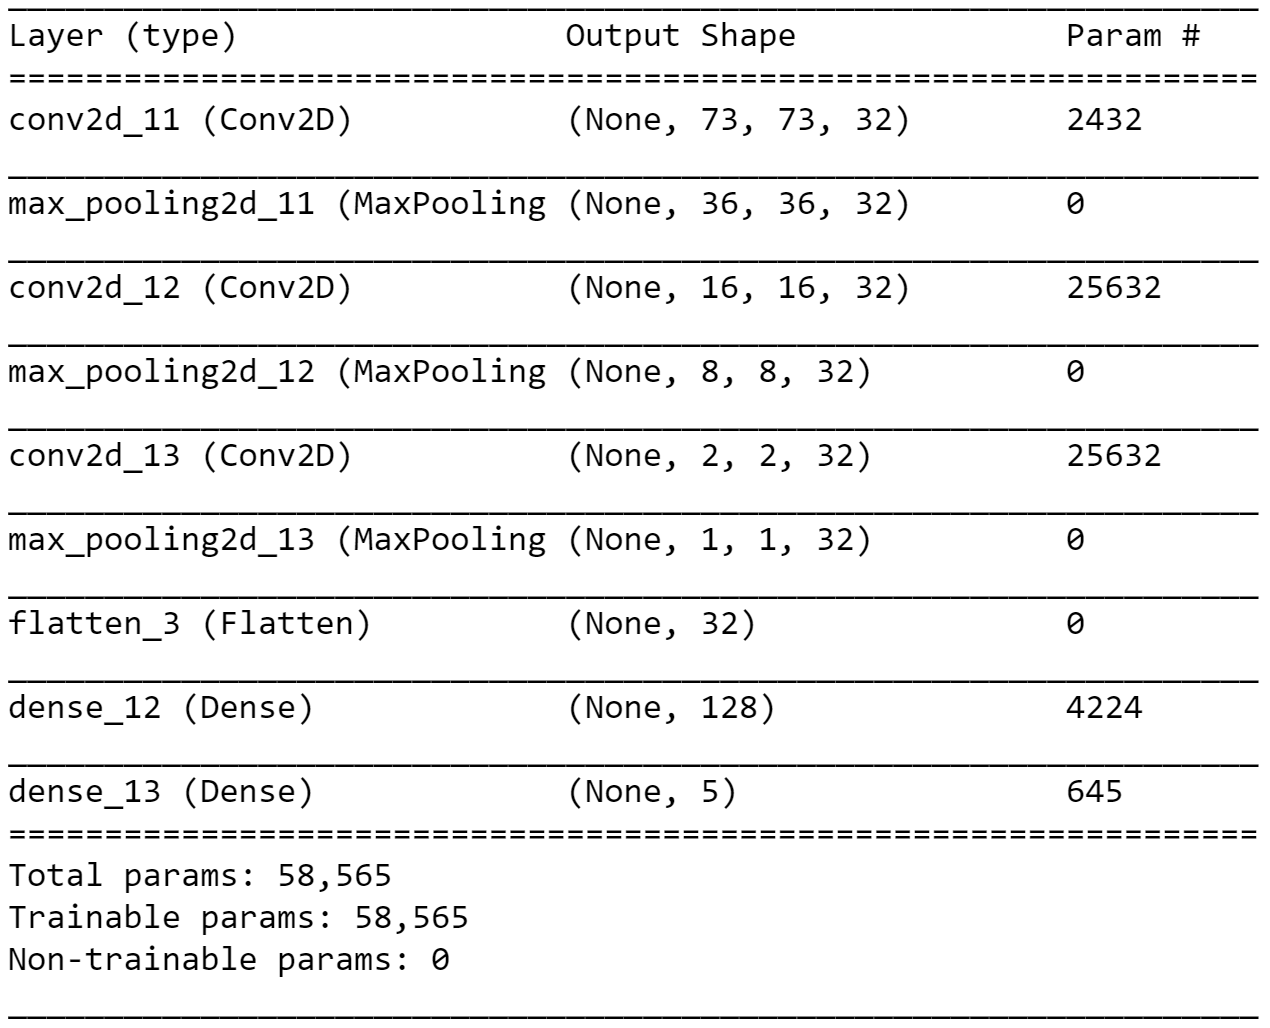
\includegraphics[scale=0.60]{../figs/model_arch/cnn_b2.png}	
\caption{CNN Model B2 Sample Architecture}
\label{fig:CNN_B2_Arch_Model} 
\end{figure}

\begin{figure}[!h]
\centering
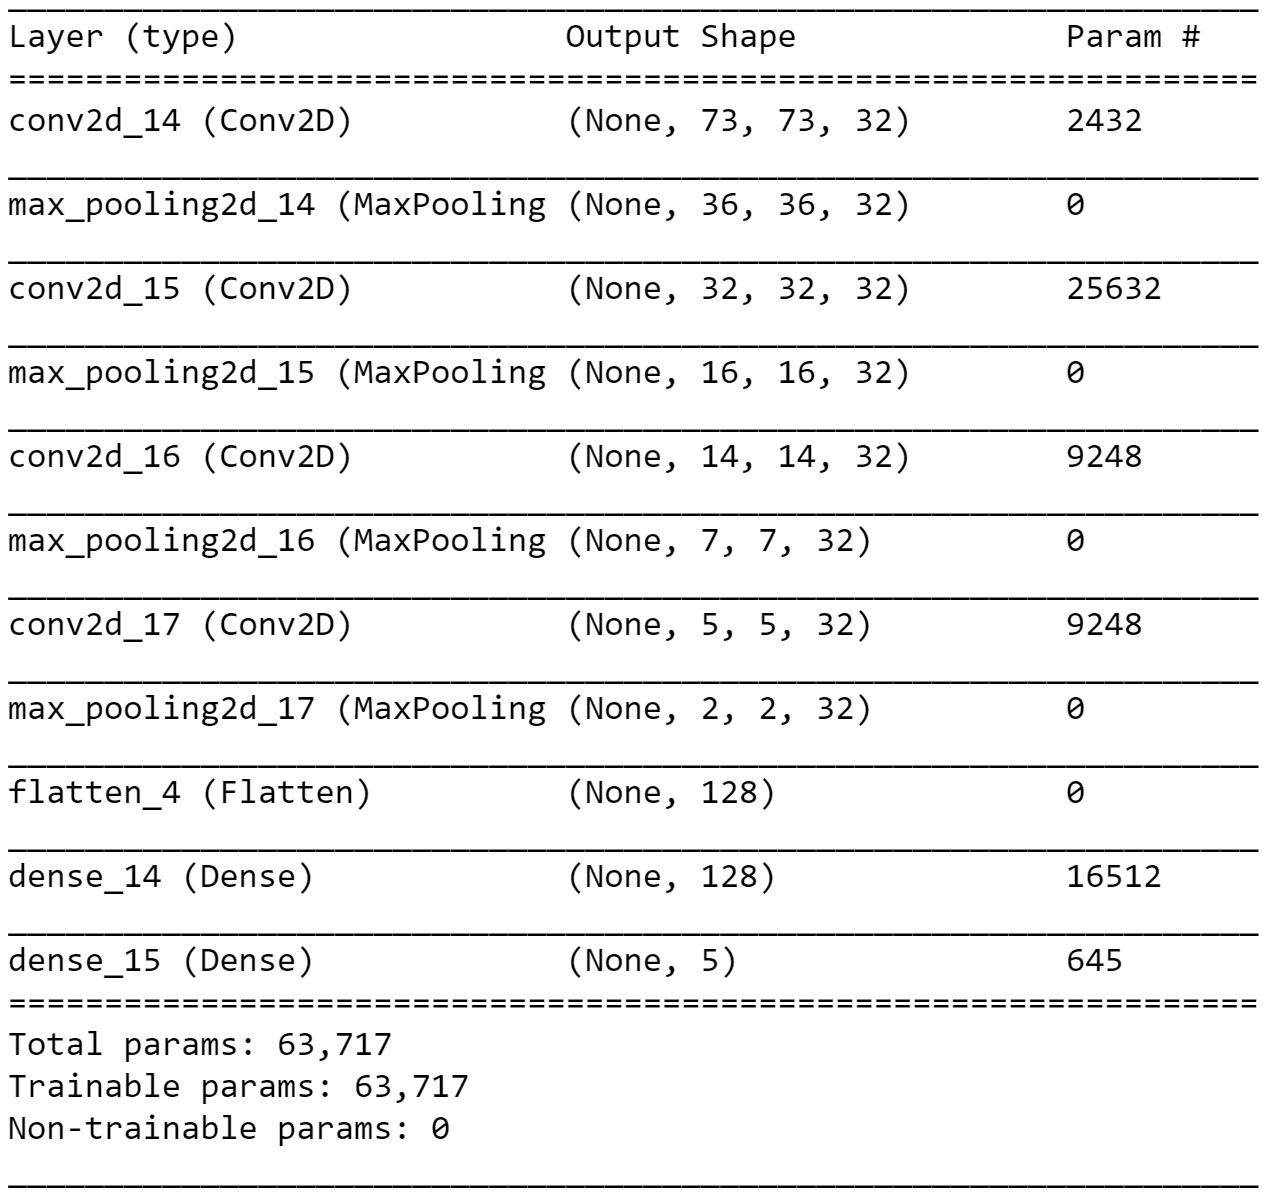
\includegraphics[scale=0.60]{../figs/model_arch/cnn_b3.png}	
\caption{CNN Model B3 Sample Architecture}
\label{fig:CNN_B3_Arch_Model} 
\end{figure}

\begin{figure}[!h]
\centering
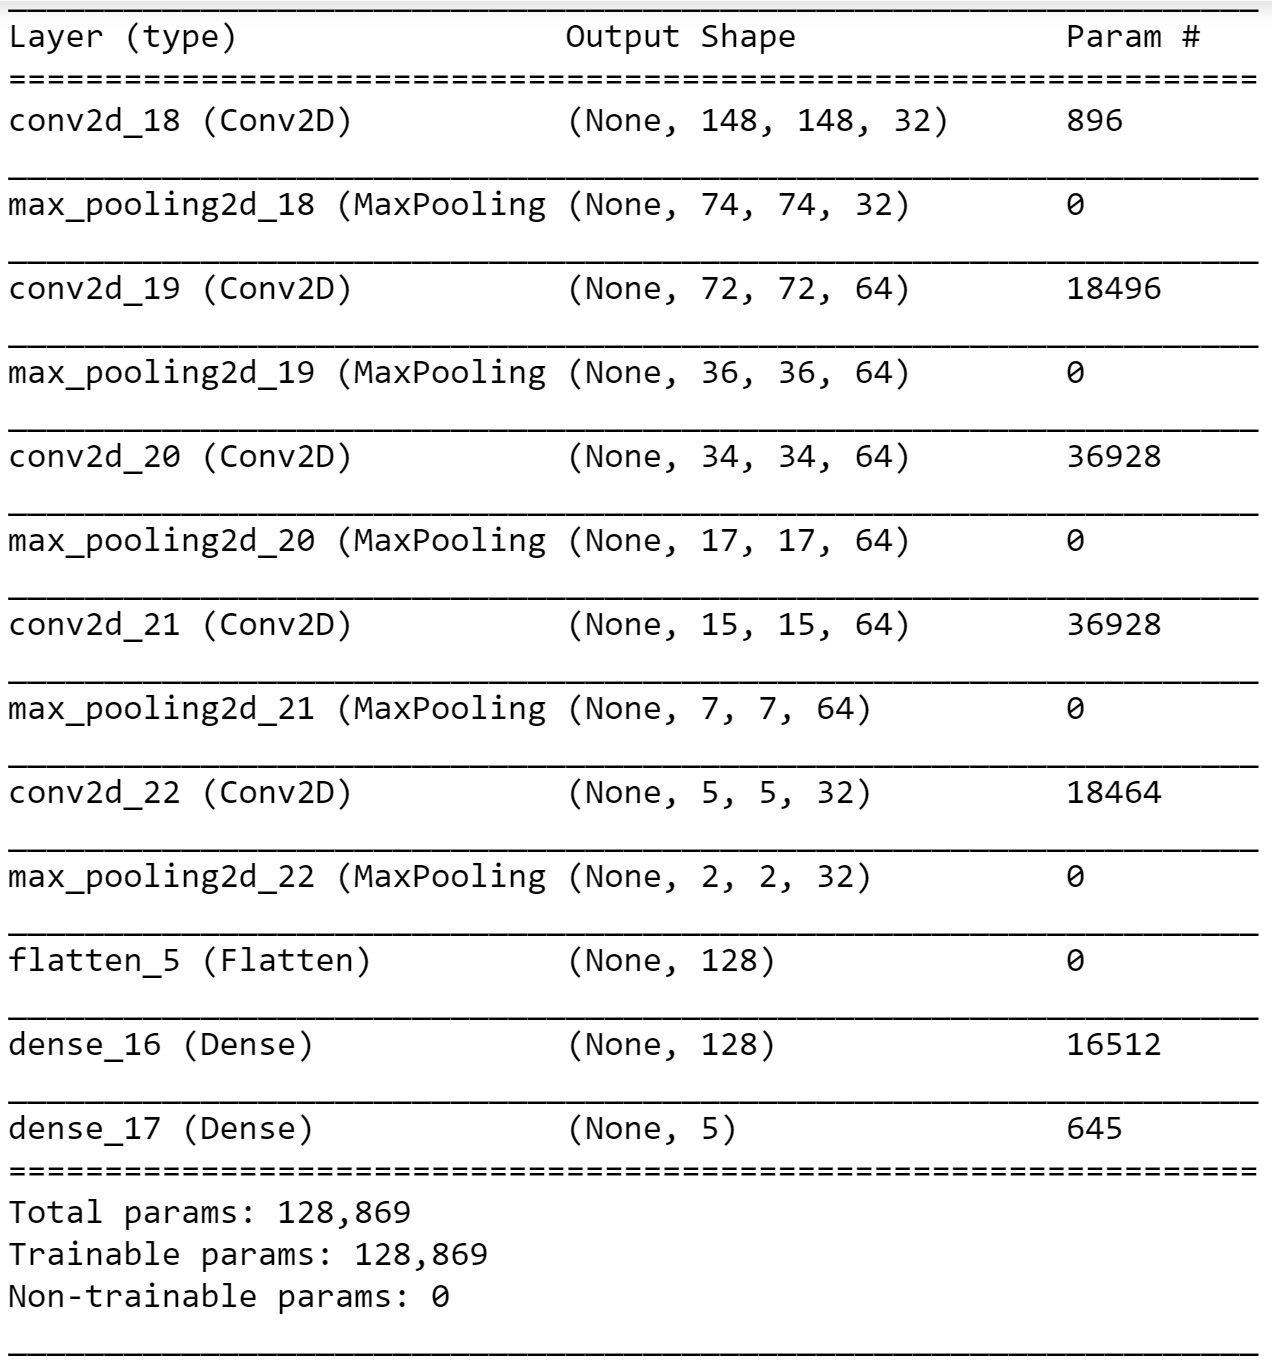
\includegraphics[scale=0.60]{../figs/model_arch/cnn_b4.png}	
\caption{CNN Model B4 Sample Architecture}
\label{fig:CNN_B4_Arch_Model} 
\end{figure}

%%%%%%%%%%%%%%%%%%%%%%%%%%%%%%%%%%%%%%%%%%%%%%%%%%%%%%%%%%%%%%%%%%%%%%%%%%%%%%%%
%%%%%%%%%%%%%%%%%%%%%%%%%%%%%%%%%%%%%%%%%%%%%%%%%%%%%%%%%%%%%%%%%%%%%%%%%%%%%%%%





\end{document}
